\documentclass[a4paper,12pt]{article}
    \usepackage[utf8]{inputenc}
    \usepackage[brazil]{babel}
    \usepackage[
        lmargin=3cm,
        tmargin=3cm,
        rmargin=2cm,
        bmargin=2cm,
        ]{geometry}
    \usepackage{indentfirst}
    \usepackage{graphicx}
        \graphicspath{{./images}}
    
    \usepackage{helvet}
        \renewcommand{\familydefault}{\sfdefault}
    
    \usepackage[document]{ragged2e}
    \usepackage{setspace}
    \usepackage{lipsum}
    \usepackage[none]{hyphenat}
    \usepackage{caption}
    \usepackage{microtype}

    % --- CITAÇÂO ABNT --- %
    \usepackage[
        alf,
        versalete,
        abnt-emphasize = bf,
        abnt-etal-list = 3,
        abnt-etal-text = it,
        abnt-and-type = &,
        abnt-last-names = abnt,
        abnt-repeated-author-omit = no
    ]{abntex2cite}
    % -------------------- %
    
    % ---------
    % VARIABLES:
    \newcommand{\ACADEMY}{
        Faculdade Senac Blumenau
    }
    \newcommand{\COURSE}{
        Graduação em Análise e Desenvolvimento de Sistemas
    }
    \newcommand{\AUTHORS}{
        Marcel E. Cattaneo \\
        Arthur Klung Junior \\
        Rodrigo Gilberto Lessa \\
        Lucas
    }
    \newcommand{\SURNAMES}{
        CATTANEO, Marcel / JUNIOR, Arthur Klung / LESSA, Rodrigo Gilberto / Lucas
    }
    \newcommand{\TEACHER}{
        Diego Pasqualini
    }
    \newcommand{\DOCTITLE}{
        como a computação em nuvem irá \\
        revolucionar o mundo dos games
    }
    \newcommand{\CITY}{
        Blumenau
    }
    \newcommand{\YEAR}{
        2022
    }
    \newcommand{\FULLDATE}{
        \CITY, 10 de Abril de \YEAR
    }
    \newcommand{\PREAMBLE}{
        \singlespacing
        \normalsize \justify Trabalho apresentado à \ACADEMY como requisito
        parcial para obtenção do título de Graduação em \COURSE.
    }
    \newcommand{\KEYWORDS}{
        1. Computação. 2. Nuvem. 3. Games. 4. Internet.
    }
    \newcommand{\DOCTYPE}{
        Trabalho Acadêmico
    }
    \newenvironment{fichacatalografica}
    {
        \thispagestyle{empty}
        \begin{singlespacing}
            \footnotesize
        \end{singlespacing}
    }

     % ---

    \title \DOCTITLE
    \author \SURNAMES
    \date \FULLDATE
    \pagestyle{myheadings}
    \pagenumbering{arabic}
    \begin{document}
        \thispagestyle{empty}
\linespread{1.5}
\begin{Center}
    \MakeUppercase{
        \bf \ACADEMY
        }
    \\
    
    \bf \COURSE
    \\

    \vspace*{1.5cm}
    \bf \AUTHORS
    \\
    
    \vspace*{5cm}
    \bf \MakeUppercase \DOCTITLE
    \\
    
    \vspace*{\fill}
    \bf \CITY \\
    \bf \YEAR
\end{Center}
        
\thispagestyle{empty}
\linespread{1.5}
\begin{Center}
    {\bf \AUTHORS}
    \\
    
    \vspace*{1.5cm}
    {\bf \MakeUppercase \DOCTITLE}
    \\
    
    % PREAMBLE
    % --------
    \vspace*{5cm}
    \hspace{.45\textwidth}
    \begin{minipage}{.5\textwidth}
        \PREAMBLE
        \singlespacing
        {\justify Orientador: \TEACHER}
     \end{minipage}
     % --------
    
    \vspace*{\fill}
    \bf \CITY \\
    \bf \YEAR
\end{Center}
        \begin{fichacatalografica}
    \linespread{1.0}
	\sffamily
	\vspace*{\fill}
	\begin{FlushLeft}
	\fbox{\begin{minipage}[c][8cm]{14.5cm}
	\small
	\AUTHORS
	
	\hspace{0.5cm} \DOCTITLE  / \SURNAMES. --
	\CITY, \FULLDATE-
	
	\hspace{0.5cm} 20 p. : il. (algumas color.) ; 30 cm.\\
	
	\hspace{0.5cm} Orientador:~\TEACHER\\
	
	\hspace{0.5cm}
	\parbox[t]{\textwidth}{\DOCTYPE~--~\ACADEMY,
	\FULLDATE.}\\
	\singlespacing
	\hspace{0.5cm}
        \KEYWORDS
		I. \TEACHER.
		II. \ACADEMY.
		III. \COURSE.
		IV. \DOCTITLE 			
	\end{minipage}}
	\end{FlushLeft}
\end{fichacatalografica}
        \thispagestyle{empty}
\linespread{1.5}
\begin{Center}
    {\bf \AUTHORS}
    \\
    
    \vspace*{1.5cm}
    {\bf \MakeUppercase \DOCTITLE}
    \\

    % PREAMBLE
    % --------
    \vspace*{4cm}
    \hspace{.45\textwidth}
    \begin{minipage}{.5\textwidth}
        \PREAMBLE
     \end{minipage}
     % --------
    
    \vspace*{4.5cm}
    \noindent\rule{6cm}{0.4pt}\\
    \TEACHER
    
    \vspace*{\fill}
    {\FULLDATE}
\end{Center}
        \thispagestyle{empty}
\begin{Center}
    {\center \bf \MakeUppercase{resumo}}
\end{Center}
    
\begin{justify}
    O estudo apresentado retrata, através de pesquisas em artigos publicados referentes ao tema principal,
     como a utilização da Computação em Nuvem abre espaço à diversos modelos Service as a Service (SaaS), 
     que possibilita diversos modelos de serviço à serem definidos e incorporados junto à nuvem, 
     onde possibilita grandes empresas do mundo dos games como a Sony, Microsoft, Nintendo dentre outras, 
     a explorarem um novo nicho de inovação, que batalha para diminuir custos ao cliente final, de forma à 
     expandir a lucratividade de forma mais horizontal, uma vez que para acessar tal tipo de serviço, o 
     cliente final não precisa comprar uma mídia física para conseguir acessar diversos títulos de jogos. 
     Conclui-se que o formato “X” as a Service será uma grande tendência em diversas áreas e é possível 
     que esta revolução chegue a tal ponto, que o cliente final sequer necessite de um console para ter 
     acesso à jogos com necessidades gráficas avançadas, em um futuro onde o entretenimento dos videogames 
     poderá ser acessado como um outro serviço qualquer, sem a complexidade de se compreender a infraestrutura 
     necessária para que tal serviço seja possível e principalmente, acessado por diversos tipos de classes sociais.
\end{justify}
{Palavras-Chave: \KEYWORDS}
\vspace*{\fill}

        \tableofcontents
        \thispagestyle{empty}
        \newpage
            
\begin{justify}
    \section{Introdução}
    A popularização do computador pessoal e do acesso à internet ao longo dos anos fomentou possibilidades inimagináveis. Com o advento da
    internet 2.0, surge um novo comportamento onde usuários começavam a ter uma prática social online de armazenar e disponibilizar fotos em
    redes sociais, criar blogs com facilidade sem necessidade de compreender como desenvolver um website ou como funciona um banco de dados,
    fomentando grandes empresas a enxergar nessa tendência que surgia na utilização da internet, modelos possível de plataforma e serviços que
    evoluiríam o acesso a este tipo de prática social de forma mais ampla. Isso evidenciou uma nova demanda por serviços onde o usuário passa a
    ser também consumidor.

    Esta evolução dependia não apenas da disponibilidade de novos tipos de serviço, mas também da evolução da infraestrutura de virtualização e
    comunicação de sistemas disponibilizados na internet para trazer ao mundo a possibilidade de manter grandes aplicações online, de forma
    escalável dando surgimento a modelos de serviços que contemplem uma forma mais ágil de acesso onde a informação precisa estar presente, ao
    alcance das mãos, independente da posição geográfica do meio de acesso, desde que este tenha os requisitos mínimos para que seja possível
    acessar o serviço que entrega praticidade e segurança ao cliente. 

    A partir dessa necessidade surge o conceito de Computação em Nuvem (CN), que de acordo com (CARISSIMI, 2015) “é um modelo de negócio
    onde um usuário paga apenas pelo o que consome de recursos (modelo pay-as-you-go) e o provedor do serviço mantém uma infraestrutura física
    ( data center )”, estrutura essa que além de trazer complexidade e poder de processamento de forma abstrata, traz também segurança, baixo
    custo e novos modelos de serviço que podem ser explorados tanto pelos usuários finais, bem como empresas que desejam disponibilizar um tipo
    de aplicação própria, como uma rede social, como um serviço. 
    Este nicho de “serviço como serviço” é definido de Software as a Service (SaaS), que consome de outros modelos de serviço relacionados à CN,
    como podemos observar na figura abaixo:
        
    \begin{Center}
    \begin{figure}[h]
        \centering
        \caption{Fonte}
        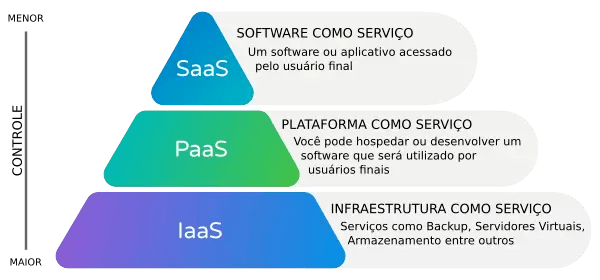
\includegraphics[scale=0.5]{iaas-paas-saas}
        \label{fig:iaas-paas-saas}
    \end{figure}
    \footnotesize{Fonte: Blog Tecnomega, 2021}
    \end{Center}

\end{justify}

\begin{justify}
    Observando a FIGURA 1, verificamos que para se disponibilizar um SaaS uma entidade depende também das estruturas de Plataforma como
    Serviço (PaaS) e principalmente da base de Infraestrutura como Serviço(IaaS), mesmo que a própria entidade seja dona de toda estrutura que o
    SaaS tenha como base, o modelo de CN se mantém o mesmo.

    Com a praticidade do acesso à estrutura CN e seus modelos de serviço deram possibilidade a surgirem também outros modelos de estrutura,
    variantes do SaaS, apenas para afirmar o tipo de serviço ofertado. Este modelo pode ser definido como “X” as a Service e é neste formato que
    grandes empresas do mundo dos games apostam para revolucionar a forma como este tipo de entretenimento pode ser mais acessível à
    diversas classes sociais, horizontalizando o acesso e aumentando a lucratividade uma vez que, o custo em se adquirir uma mídia física contendo
    um títilo de jogo, ou até mesmo no futuro, a necessidade a ter um hardware robusto e caro, fica amortizado pela própria plataforma que
    disponibilizará o possível Game as a Service (GaaS).
\end{justify}
            \begin{justify}
    \section{Objetivos Específicos}

    \begin{itemize}
        \item Dar breve introdução ao modelo de Computação em nuvem;
        \item Determinar as vantagem da Computação em nuvem.
        \item Elucidar o modelo Game as a Service (GaaS), apontando vantagens nesta nova abordagem.
    \end{itemize}

\end{justify}

            \begin{justify}
    \section{O que é Computação em Nuvem?}
    Segundo Rachid (2019), a computação em nuvem não se enquadra em ser apenas um
    pedaço de tecnologia como um celular ou um computador, ela nada mais é do que um
    sistema online que disponibiliza serviços ao usuário usando como meio de distribuição a
    internet e se divide em três braços: infraestrutura como serviço, software como serviço e
    plataforma como serviço.

    A computação em nuvem utiliza hardware (parte física dos recursos de computação) e
    software (parte de digital, de controle das partes físicas) para entregar serviços que podem
    ser acessados de inúmeros dispositivos conectados à rede. Essa computação sob demanda
    visa compartilhar recursos de computação como processamento e armazenamento.
    Alguns desses serviços podem ser de compartilhamento de vídeos como
    “NETFLIX”, com seu catálogo de filmes e séries, o google com o youtube e o gmail, e
    muitos outros serviços acessados hoje pela internet, recursos do cloud computing.

    O que uma empresa necessita para funcionar? Armazenamento de dados, integração com
    filiais, gerenciamento de recursos, gerenciamento de pessoas, essa integração pode ocorrer
    hoje por dois meios, a empresa pode ter sua própria estrutura de recursos como softwares e
    hardwares para implementação desses requisitos de funcionamento, ou pode ser pela
    nuvem. A ideia inicial de serviços pela nuvem é a segurança dos dados, rapidez de colocar
    tudo para funcionar e menor custo de implementação.

    \vspace{0.2cm}
    \begin{flushright}
        \begin{minipage}{.7\textwidth}
            \noindent
            \footnotesize
            \setstretch{1.0}

            \begin{justify}
            Bem, podemos dizer que a Computação em Nuvem é um termo para descrever um
            ambiente de computação baseado em uma imensa rede de servidores, sejam estes
            virtuais ou físicos. Uma definição simples pode então ser “um conjunto de recursos
            como capacidade de processamento, armazenamento, conectividade, plataforma,
            aplicações e serviços disponibilizados na internet”. O resultado é que a nuvem pode
            ser vista como o estágio mais evoluído do conceito de virtualização, virtualização do
            próprio data center. \cite{taurion2009cloud}
            \end{justify}
        \end{minipage}
    \end{flushright}
    \vspace{0.2cm}

\end{justify}


\begin{justify}
    Os recursos de hardware físico geralmente não são baratos de se implementar, onde então
    entra a nuvem, à qual oferece inúmeros serviços online como processamento de dados,
    armazenamento, conectividades e até sistemas completos para empresa funcionar, que
    ficam disponíveis 24h por dia, 7 dias por semana em servidores físicos ou servidores
    digitais. \cite{rashid2019cloud}

    \subsection{INFRAESTRUTURA}
    No quesito de infraestrutura a computação em nuvem disponibiliza diversos modelos de
    hardware para uso online, ela utiliza a virtualização de recursos físicos e os disponibiliza
    para o consumidor, fazendo com que recursos físicos sejam dinamicamente convertidos em
    recursos lógicos de acordo com o uso. Tais recursos podem ser de processamento (CPU),
    memória (RAM ou de armazenamento), completos sistemas operacionais (windows, linux) e
    softwares de aplicação. \cite{pedrosa2011computaccao}

    Os benefícios de utilizar esse tipo de serviço são inúmeros, por exemplo o custo desses
    serviços online são bem mais baratos do que adquirir esses recursos físicos, os usuários
    pagam apenas aquilo que quiserem usar e o usuários pode optar por upgrades e
    downgrades nos serviços a qualquer momento.

    \subsection{PLATAFORMA}
    Com o serviço de plataforma o cloud pode hospedar tanto o software usado quanto às
    especificações de hardware necessárias para rodar tal aplicação, usando assim pouco
    requerimento de hardware e software do usuário, gerando assim uma facilidade de acesso
    de diversos dispositivos a aplicação. Conforme o usuário “compra” o direito de usar uma
    aplicação ele já paga por todo o requerimento necessário para rodar a aplicação.

    Os benefícios desse tipo de serviço são várias, por exemplo uma empresa pode comprar
    um software gerenciado por cloud e com isso ter segurança e acesso de qualquer unidade
    ao mesmo banco de dados, sem a necessidade de investir no seu próprio banco de dados e
    com um investimento mínimo de equipamentos para rodar essas aplicações direto na
    nuvem.\cite{rashid2019cloud}

    \subsection{SOFTWARE}
    Os serviços disponibilizados pela cloud podem ser diversos, desde o gmail da google até
    um sistema inteiro de gerenciamento de uma multinacional. Cada provedor de serviços via
    nuvem se responsabiliza pela segurança dos dados do seu cliente e por manter o serviço
    online, atualizações e problemas encontrados pelos usuários são de responsabilidade do
    próprio provedor do serviço. \cite{taurion2009cloud}

    Essa área da cloud é a mais utilizada pelo usuário final. Serviços de streaming de vídeo,
    jogos e qualquer outra aplicação que o usuário acesse de seu smartphone, computador ou
    qualquer dispositivo ligado a rede de internet, são mantidos online por algum responsável
    por distribuir tal tipo de serviço.

    \subsection{RECUPERAÇÃO}
    Cada serviço disponibilizado pela computação em nuvem, tem um sistema de backup, que
    armazena e faz backups dos dados dos usuários, fazendo com que o usuário não perca
    nenhum de seus dados e arquivos.\cite{rashid2019cloud}

    \subsection{JOGOS DIGITAIS}
    Segundo \cite{huizinga1971homo} os jogos são uma atividade lúdica que se utiliza de fenômenos
    físicos, psicológicos e é o ato voluntário de retirar o participante da vida real, adicionando
    uma tensão ao participante por não saber como será o desfecho do jogo.

    Um jogo apresenta quatro pilares fundamentais para sua criação, a representação do jogo
    que oferece ao jogar um mundo completo sem a necessidade de depender de algo do
    exterior e um completo conjunto de regras e definições para ser jogado, a interação onde o
    jogador pode realizar ações que alteram o desfecho do jogo e pode analisar o que sua ação
    resultou, o conflito que são ações que o criador do jogo criou para dificultar com que o
    jogador conclua de forma fácil o jogo tais como barreiras a serem quebradas ou um
    cronômetro e por fim a segurança que o jogador está seguro de riscos físicos de suas ações
    no jogo nao quer dizer que o jogador sairá ileso porém pode perder benefícios dentro do
    jogo. \cite{crawford1984art}

    \section{Captando dados e construção de Persona}

    Com o advento da Computação em Nuvem diversos serviços do tipo \textit{Service as a Service}
    começaram a serem fomentados uma vez que agora grande coorporações tem a possibilidade de
    escalonar até mesmo a infraestrutura, pagando apenas pelo que o serviço irá consumir. Com novos
    serviços surgindo a internet passa a ser um meio que vei além da comunicação para adentrar no
    mundo da Internet das Coisas que, de acordo com \cite{albertin2017internet} pode ser
    compreendida como uma rede global que auxilia na integração do mudo virtual com o mundo físico,
    bem como com equipamentos diversos e até mesmo sensores que podem captar e armazenar dados,
    deixando estes salvos para um possível interesse corporativo de alguma empresa, prestadora de um
    serviço especifico.

    Este tipo de pratica não só é útil ao cliente como principalmente para a entidade que fornece
    o serviço uma vez que, cruzando dados préviamente armazenados e com o concentimento do cliente à
    nivel contratual do serviço, fazem com que seja possível mapear comportamentos, tendências e até
    mesmo uma escolha futura para o cliente, fazendo com que vendas sejam ainda mais efetivas e o
    cliente nesse contexto, se satisfaz ao receber uma possível recomendação de algo que tendenciava
    a adquirir ou a uma ação que possivelmente iria tomar.

    Com este nível de acesso à informaão dos cliente, empresas que fornecem serviços do tipo
    textit{SaaS} começaram a montar a textit{persona} dos cliente, mantendo uma relação que pode ser
    dita até mais íntima onde segundo \cite{dospersona}, deve ser criada uma persona, a partir da
    coleta de dados e informações úteis que auxiliem na compreensão comportamental do cliente. Isto
    fez com que a concorrência entre as empresas de cativar o cliente, fosse também em baseada nos
    dados que estas conseguem captar em seus próprios serviços.

    \subsection{Game as a Service, aproximação com os clientes}

    Não é de hoje que existe uma disputa acirrada entre as gigantes do mundo dos games, é notável
    por exemplo a concorrência entre a Sony e a Microsoft para manterem seus usuários entretidos
    ofereendo cada uma delas títulos exclusivos com a ideia de uma possível fidelização do
    cliente. Para jogar um determinado título ofertado exclusivamente por uma empresa, o cliente
    deveria adquirir o console desta, bem como a mídia física do título. Este modelo de aquisição
    acabava segregando as possibilidades dos clientes onde estes atualmente optam por um console
    apenas e investem um montante expressivo de dinheiro para conseguir jogar.

    Com a evolução da estrutura da internet e sua capacidade de transmitir dados junto ao novo
    modelo de serviço SaaS gerando novas tendências de mercado, à exemplo de grande empresas de
    textit{streaming} de filmes e séries que deixaram a mídia física dos filmes obsoletas e
    entendendo que a luratividade está na fidelização do pagamento e nao apenas na venda de mídias,
    as empresas de games começaram a explorar o que podemos chamar de modelo textit{Game as a
    Service} que tenta seguir com uma assinatura mensal para o cliente ter acesso, onde o valor da
    assinatura é mais suave do que o montante necessário na aquisição da mídia física.

    Atualmente empresas como Microsoft, Sony, EA dentre outras, optaram em apostar no modelo
    textit{GaaS} um vez que este além de ser lucrativo, oferece ao cliente um valor baixo para
    conseguir acessar diversos jogos originais fazendo com que este não busque meios alternativos e
    piratas para conseguir jogar em um console desbloqueado, que para as empresas de game, pode ser
    considerado um console morto e um cliente que não consome da fonte original.
    O modelo textit{GaaS} de serviço pode tambem ser considerdo um serviço textit{Over The Top} que
    encontra-se, segundo \cite{tristao2020pirataria} voltado para os clientes terem acesso a uma
    infinidade de conteúdos digitais, a preço de custo acessível dentre os padrões atuais, podendo
    ser considerado um valor muito abaixo das mídias físicas.

    Este tipo de serviço fideliza mais clientes de diversas classes sociais que antes optavam por um
    meio alternativo, principalmente em países de terceiro mundo onde a fiscalização é bastante
    fraca e este modelo de lucro à partir de direitos autorais mostrou-se antiquado ao surgimento
    dos modelos textit{XaaS}.

    \section{Conclusão}
    Portanto é possível entender que a evolução da internet bem como do computador pessoal, trazendo
    novas possibilidades de serviço que fometaram uma evolução profunda junto a estrutura
    da computação, criando enfim o que chamamos de Computação em Nuvem, que por sua vez deu início a
    uma gama de possibilidade de processamento e armazenamento de dados para ofertar serviços onde o
    cliente paga apenas pelo que consome e não mais adquire uma licença para a utilização de um
    software, por exemplo.

    Este modelo impactou na forma como as empresas ofertam produtos, muitas delas optaram em
    transformar seus produtos em serviços virtuais para ampliar de forma horizontal, a cartela de
    clientes, almejando lucratividade a medida que o acesso ao serviço se dá mediante a uma
    assinatura em que o cliente poderá assinar ou cancelar a qualquer momento.
    Desta forma, surgem vertentes do modelo SaaS que é o topo da pirâmide (FIGURA 1) da Computação
    em Nuvem, que agregam outros tipos de serviço de forma genérica, que não sejam voltados
    exclusivamente à computação, como o caso do modelo textit{GaaS}.
    
    Por sua vez o modelo textit{GaaS} é benéfico tanto para as empresas como para os clientes pois o
    baixo custo da assinatura deste modelo é atrativo aos clientes que não mais optam por meios
    alternativos para ter acesso a um título, como por exemplo através de jogos pirata e consoles
    desbloqueados, além disso o cliente consegue jogar diversos jogos desde que pague uma
    assinatura, que compensa à longo prazo dado o valor absurdo das mídias físicas.


\end{justify}
        \newpage
        \section{Referências}
        \bibliographystyle{abntex2-num}
        \bibliography{references.bib}
    \end{document}
